\chapter{Introduction to SDN based Application}

\section{Introduction to Floodlight}
Floodlight is an open source java-based SDN controller and was the controller of choice for this project because of reasons such as - it supports switches which are OpenFlow enabled, it is Apache licensed and can be used for almost any purpose, it has good documentation and a very active community of professional developers who were able to resolve any issues that we needed help with.


\section{Floodlight Architecture}
\begin{itemize}
\item OpenFlow – works with physical- and virtual- switches that speak the OpenFlow protocol
\item Offers a module loading system that make it simple to extend and enhance. 

\item Open community – Floodlight is developed by an open community of developers. It welcomes code contributions from active participants and openly share information on project status, roadmap, bugs, etc.

\item Easy to Use- Floodlight is drop dead simple to build and run. Read through the Documentation (link)

\item Tested and Supported – Floodlight is the core of a commercial controller product from Big Switch Networks (link) and is actively tested and improved by a community of professional developers


\end{itemize}
    
\begin{figure}[h]
\caption{Floodlight Architecture}
\centering
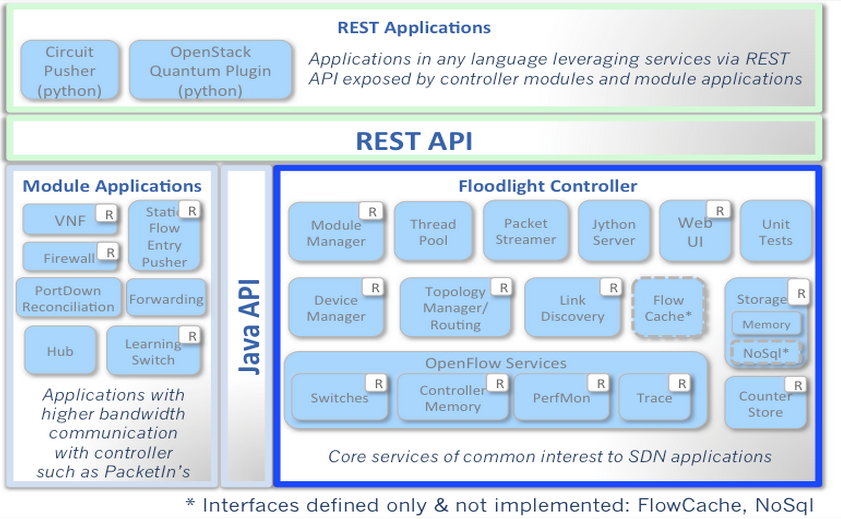
\includegraphics[width=0.9\textwidth]{Floodlight_architecture}
\end{figure}

\section{Baadal Sandbox setup}
For testing the simulation of the application, we need an environment like baadal. Baadal sandbox provides an environment by replicating actual Baadal architecture and configurations. It is fast and easy way to test the solution of network virtualisation. 



\begin{figure}[h]
\caption{Setup of Baadal Sandbox Installed }
\centering
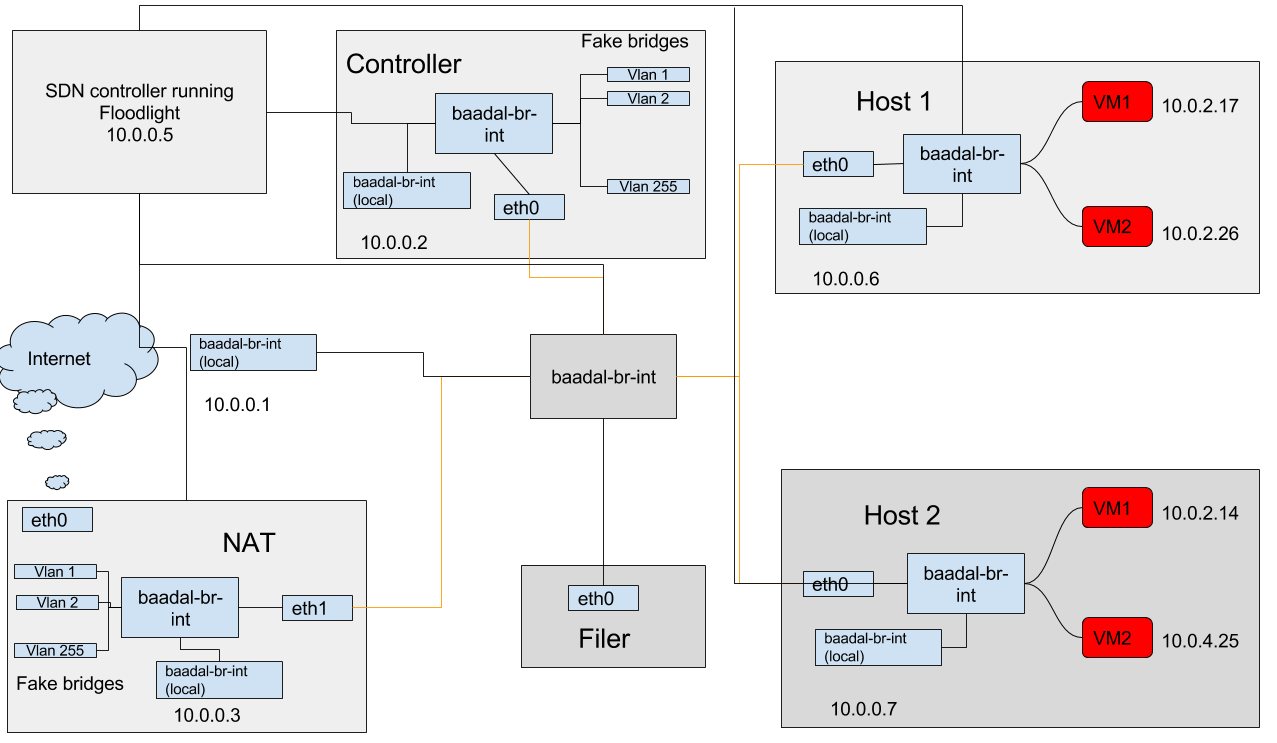
\includegraphics[width=0.9\textwidth]{baadal_networking_diagram}
\end{figure}

If tested successfully, we can subsequently deploy the solution in actual Baadal with some modifications.

The differences with which sandbox mimics baadal architecture are:-

\begin{itemize}
    \item Physical hosts, baadal controller, filer, NAT are implemented as VMs on a single physical machine
    \item OVS is the switch used for implementing hardware switches
    \item All the VMs are implemented into the physical hosts which makes two level of virtualisation
\end{itemize}



\section{Inter-VLan Issues and Modifications suggested}

\subsection{How do VMs communicate?
}
In the existing
Baadal network as explained above, the inter VM communication takes place
as follows:


\begin{itemize}
   
    \item \textbf{VMs in same host and same VLAN/subnet} In this case, the OVS bridge
in the host would simply be able to let them communicate by learning their
mac-port pair as they fall in the same broadcast domain. 

\begin{figure}[h]
\caption{Routing in Same Host and Same VLAN}
\centering
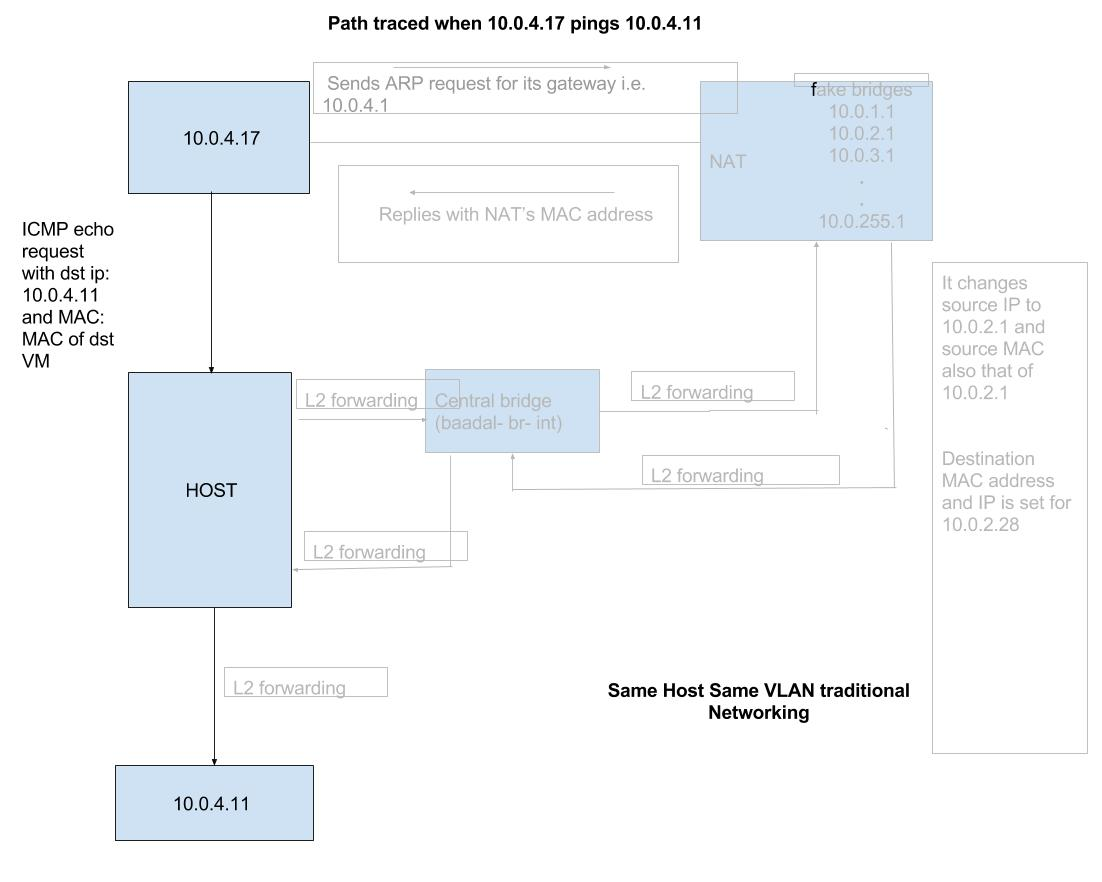
\includegraphics[width=0.9\textwidth]{Samehost_SameVLAN}
\end{figure}

The VLAN
tag corresponding to the VLAN will be attached at the ingress port while
the egress port will strip it off before sending the packets out.


\pagebreak



     \item \textbf{VMs in different host but same VLAN/subnet} In this case, still, the broad-
cast domain is the same. So, in addition to the host OVS bridge, the
central switch will come into picture. The process will be same as above
case except for the extra central switch through which the packets would
travel.

\begin{figure}[h]
\caption{Routing in Same Host and Same VLAN}
\centering
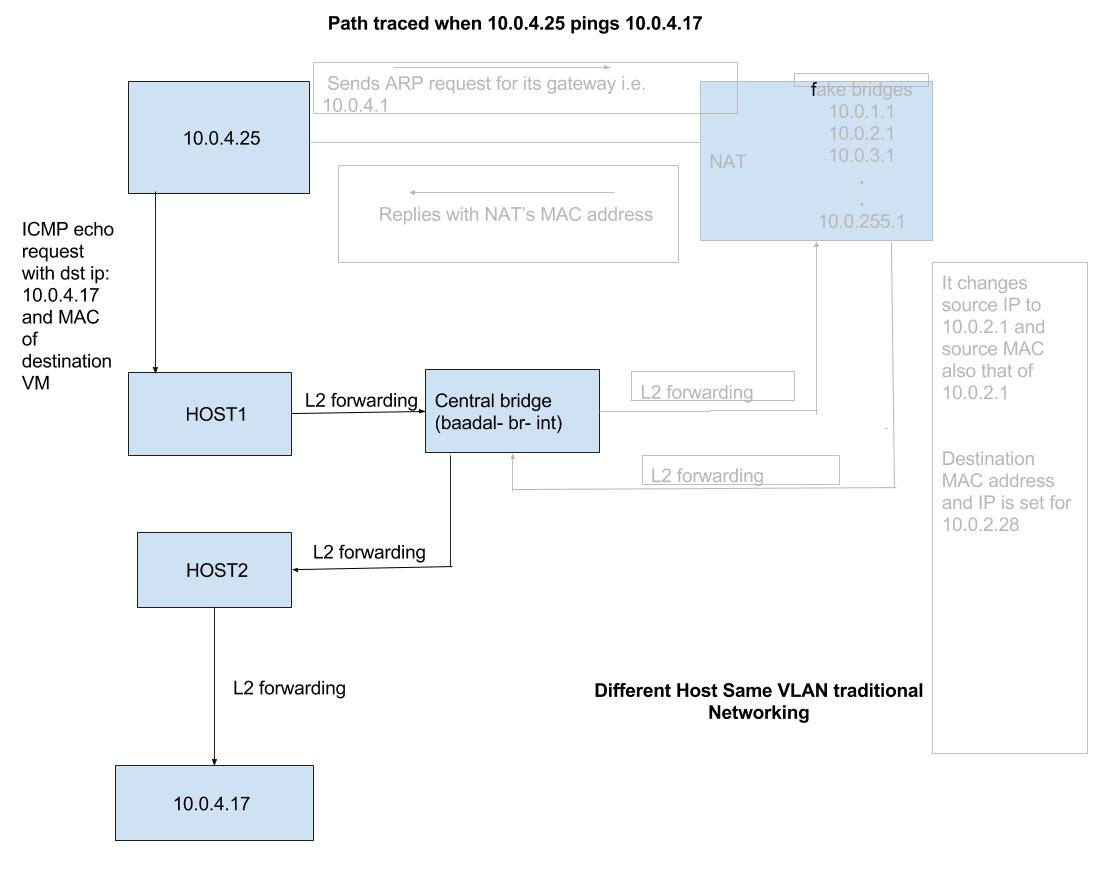
\includegraphics[width=1.0\textwidth]{Differenthost_sameVLAN}
\end{figure}

\pagebreak

      \item \textbf{VMs in the same host but different VLANs/subnets}The host OVS bridge,
in this case, would not be able to forward the packets as the broadcast
domains are different. As the gateway is fake bridge for that VLAN, the
packets go all the way up to the NAT machine passing through the central
switch. The fake bridges functions to modify the VLAN tag from the in-
put VLAN to the output VLAN. The modified packets are then forwarded
at the appropriate port of NAT OVS bridge and then they come back to
the same host. Finally, the OVS bridge in the host strip off the VLAN
tag and send it out the appropriate port.

\begin{figure}[h]
\caption{Routing in Same Host and Different VLAN}
\centering
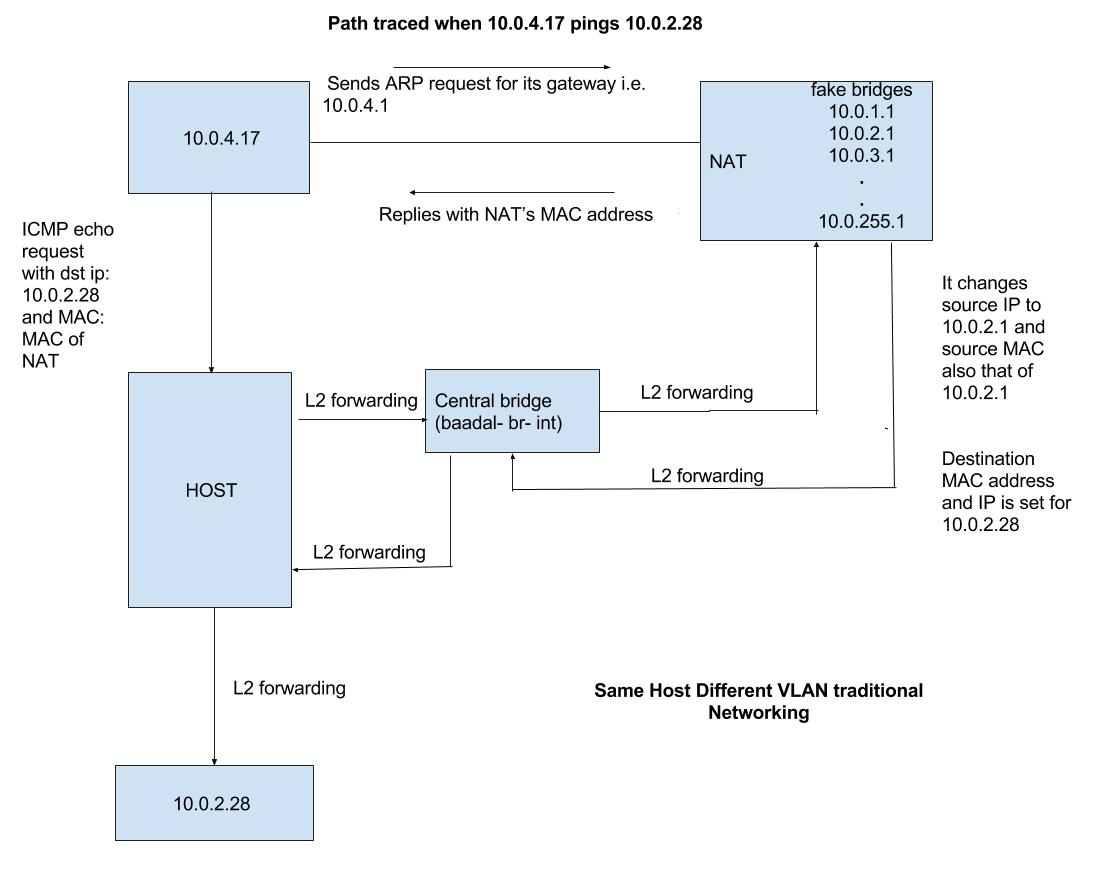
\includegraphics[width=1.0\textwidth]{Samehost_differentvLan}
\end{figure}

\newpage

\item \textbf{VMs in different hosts and different VLANs/subnets} the process is ex-
actly similar as in the previous case. The only change - different destina-
tion host - would be taken care off by the central switch as a part of its
normal l2-learning functionality.

\begin{figure}[h]
\caption{Routing in Different Host and Different VLAN}
\centering
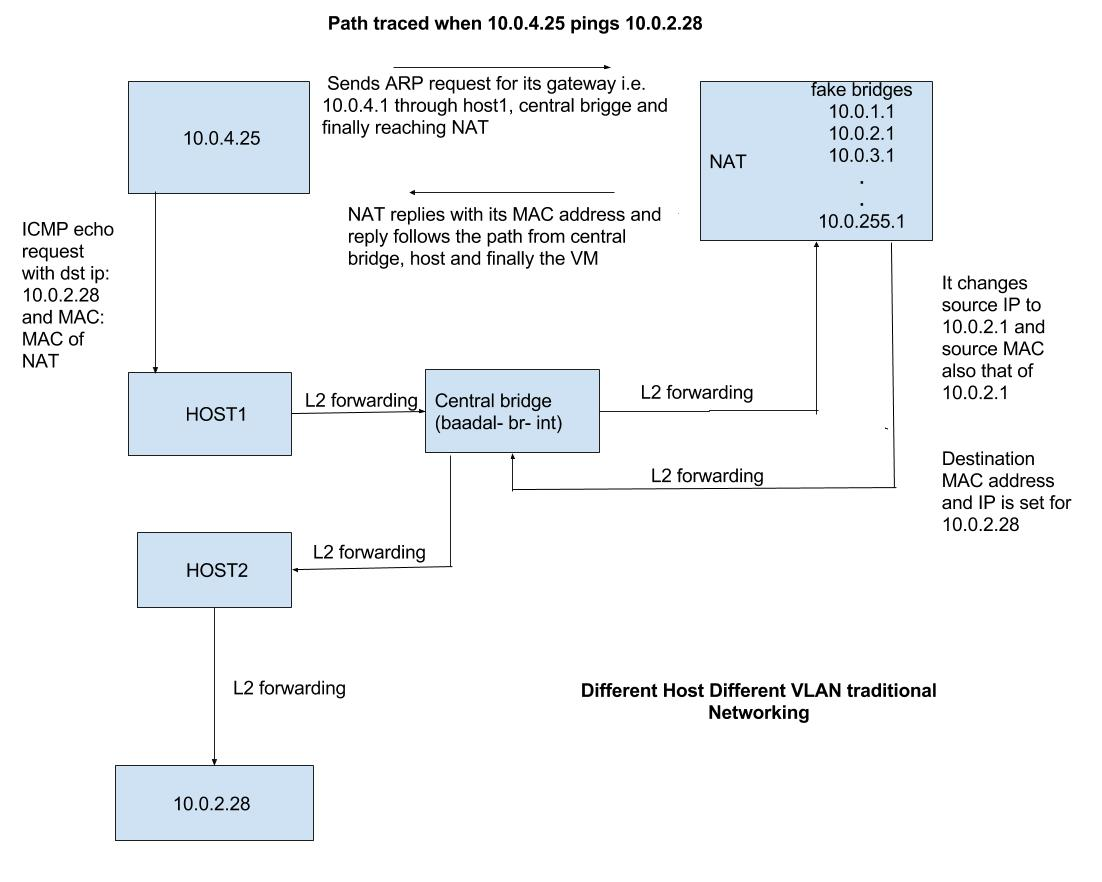
\includegraphics[width=1.0\textwidth]{Differenthost_differentvLan}
\end{figure}

\end{itemize}

\pagebreak 

\subsection{Limitation in present architecture}
We find the following limitations in the present architecture.

\begin{itemize}
\item Inter-VALN or subnet routing In the above architecture, fake bridges are
used as the mean to enable this feature. The issue is when VMs in the
same host but different subnet want to communicate. The packets have to
go all the way upto NAT machine and come back. This seems unnecessary
strain on the network and large latencies.

\item  Controlling inter-VALN routing Currently, there is no way of turning VLAN
routing on or off in Baadal. It is enabled by default. A granular level control of this feature with the current network architecture seems non-trivial
and difficult to implement



\item Maximum number of VLANs This architecture has an upper boung of 255
VLANs because of the one to one correspondence between the subnets
and the VLANs.


\item Number of VMs in a VLAN The number of VMs in each VLAN in the cur-
rent implementation is upper bound at 255. This is when considering the
addressing scheme of 192.168.x.y or 172.16.x.y with 255x255 addresses
available.

\end{itemize}

\subsection{Modification in Network Architecture}
We proposed and implementing the following modifications in the network architecture.

\begin{itemize}
    \item \textbf{No subnets} The reason subnets are used is because they define the broadcast
domains. The domains restrict the hops that broadcast packets travel and
helps in controlling traffic volume in network. But, with a SDN controller
application, the same thing could be acheived without having the subnet
restriction. The reason we want to remove it is bacause the fake bridges
are required only to enable inter subnet routing. Fake bridges being in
NAT requires packet to cover all the way upto NAT and back. Thus,
with just one subnet, the local OVS bridges would be able to forward the
packets.
\item \textbf{VLANs implemented using VLAN tags only} As opposed to having both
subnets and VLAN tags to implement VLANs, we use only VLAN tags.
The IEEE 802.1q protocol provides 12 bit VLAN tag amounting to 4094
tags. This would enable us to have 4096 VLANs as opposed to just 255!
We can further extend this to even larger numbers if we use both inner
and outer VLAN tags. Note that the VMs and the hosts are not VLAN
aware in the current as well as the proposed network architecture.

\end{itemize}

\section{Introduction to Policy routing application}
The virtual machines running in Baadal are allotted a security domain (a vlan) to segregate traffic of a certain vlan from other vlans. With using the traditional networking approach there is no way to disable it (inter-vlan routing is disabled by default in Baadal). With the SDN solution we have the capability to enable or disable it using a REST API. Moreover, there is also a provision for enabling/disabling communication between two virtual machines irrespective of their security domain. The use case for this feature would be a scenario in which people working with virtual machines in different vlans (because of them being in different departments or areas of the campus) need to collaborate with each other.

\section{Application that we are working on: Functionalities}

The application that we are working on implements modified network architecture as suggested above. The important tasks that will be handled in the application are as follows:

\begin{itemize}
    \item Tagging the packets if they ingress at an access port in a host and egress
from the trunk port.
\item Untagging the packet when they are to egress to an access port and they
have a tag attached

\item The application handles ARP and DHCP packets which are special kind
of packets. The details of how it is being done is presented in the following
sections.

\item The application takes care of security by restricting which kind of packets
reach where.

\item It takes care of forwarding normal traffic from one node to other.

\item It handles inter-VLAN routing as well.




\end{itemize}



\section{Floodlight modules}
Floodlight has modular architecture to implement any application over it and control its features. There are two kind of modules in floodlight
\begin{itemize}
    \item \textbf{Controller Modules} these implement core network services a software defined network should expose to applications
    \item \textbf{Application Modules} these implement solutions for different purposes like firewall, static flow pusher, L2 learning switch etc.
\end{itemize}

Module loading system has a JAVA interface IFloodlightModule that realises this framework.
\subsection{Module Loading System} The following are the objectives of the this system
\begin{itemize}
    \item What are the modules that are to be loaded using a configuration file
    \item Modify the implementation of modules without affecting other modules that are dependent on them
    \item Creating a platform and API to extend Floodlight
    \item Code Modularity is enforced
    \end{itemize}
The main parts of this system are 
\begin{itemize}
    \item \textbf{Modules} It is a class that implements the IFloodlightModule interface
    \item \textbf{Services} these are the services that the module provides. these are implemented as interface that extends the IFloodlightService interface
    \item \textbf{Configuration file} It contains the modules that are to be loaded
    \item \textbf{module file} It contains list of all classes used by JAVA service loader  
\end{itemize}

\subsection{How to write a Module} Following are main steps for writing a Floodlight Module
\begin{enumerate}
    \item Add a class to implement IOFMessageListener and IFloodlightModule interfaces
    \item Import Module Dependencies and set up Initialization
    \item Register a listener for PACKET\_IN Messages
    \item Ordering the modules for processing OpenFlow Messages before or after a particular module as required by the application
    \item Register the module in configuration file to load the module on startup
\end{enumerate}
    
\subsection{Module: Baadal}
It implements IOFMessageListener, IFloodlightModule, and IBaadalService. The data structures used are
\begin{itemize}
    \item \textbf{gateways} list of ipv4 addresses for routing between different subnets.  
    \item \textbf{ipToTag} stores mapping of ipv4 addresses to VLAN tags
    \item \textbf{interVmPolicy} Stores the status(enabled or disabled or default) of policy routing between a pair of VMs
    
\end{itemize}

The main functions implemented are 

\begin{itemize}
    \item \textbf{processPacketIn()} sends the packet for processing according to the source switch that it is coming from
    \item \textbf{init()} initialises variables and data structures (ipToTag, interVmPolicy etc.)
    \item \textbf{TimerTask()} schedules a task to clear cached entries in data structures at regular intervals
    \item \textbf{getIpToTag()} it returns mapping between IP address and corresponding VLAN tag
    \item \textbf{addIpToTag()} adds entries for mapping between IP address and VLAN tag
    \item \textbf{getInterVmPolicy} it returns the status of policy control for different pair of VMs
    \item \textbf{addInterVmPolicy} it adds entries into inter VM policy table as per requirement
    
\end{itemize}

\section{How do VMs communicate after implementation of application}

After running the policy control application, the modifications in the routing of different cases are  


\begin{itemize}
    \item \textbf{Same host and same VLAN} In this case routing design will be same as per traditional routing in baadal where the host will simply forward the packet based on the MAC address.
\end{itemize}


\begin{figure}[h]
\caption{Routing in Same Host and Same VLAN using SDN}
\centering
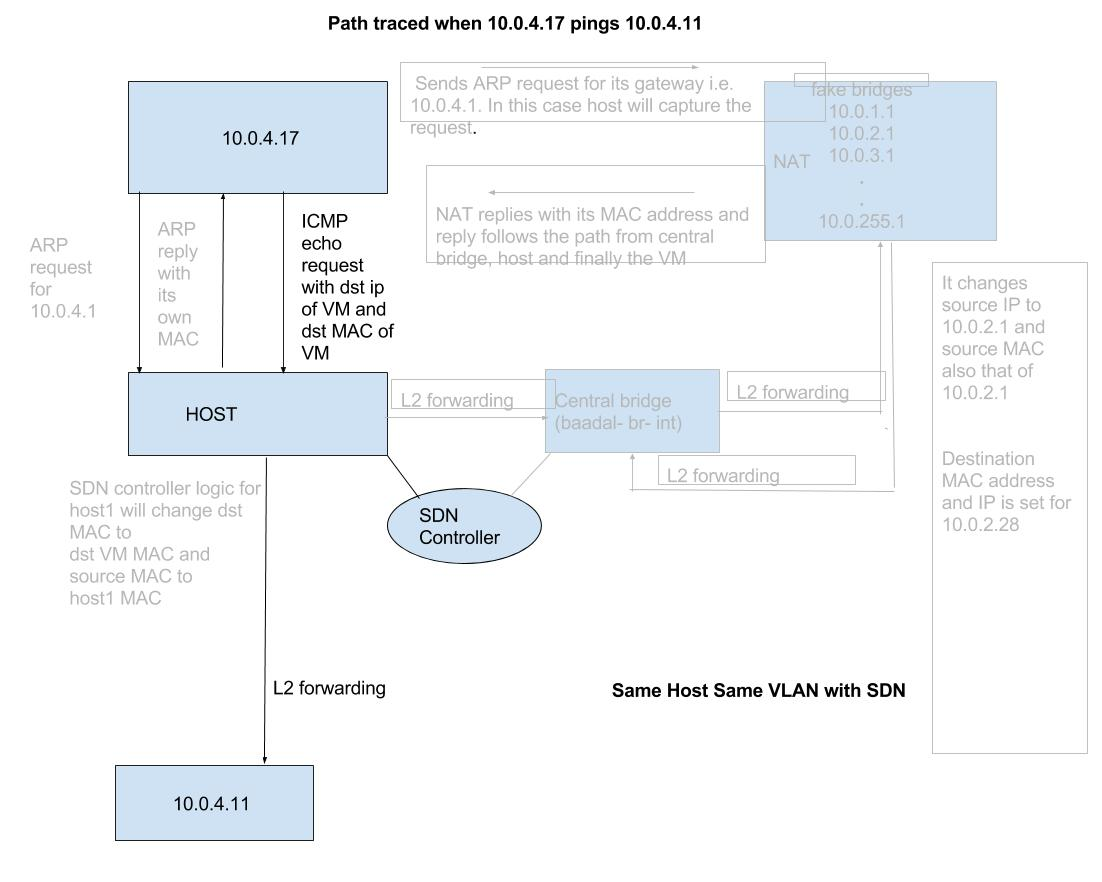
\includegraphics[width=0.9\textwidth]{Samehost_SamevLan_SDN}
\end{figure}

\pagebreak 

\begin{itemize}
    \item \textbf{Same host and Different VLAN} In this case host itself will reply to the ARP request, sent by the VM for its gateway. In traditional routing, this reply was generated by the NAT. Now the host will forward the packet to the destination VM by changing the ethernet frame (setting the destination MAC address to Destination VM MAC address and Source MAC address to MAC address of the host)
\end{itemize}

\begin{figure}[h]
\caption{Routing in Same Host and different VLAN using SDN}
\centering
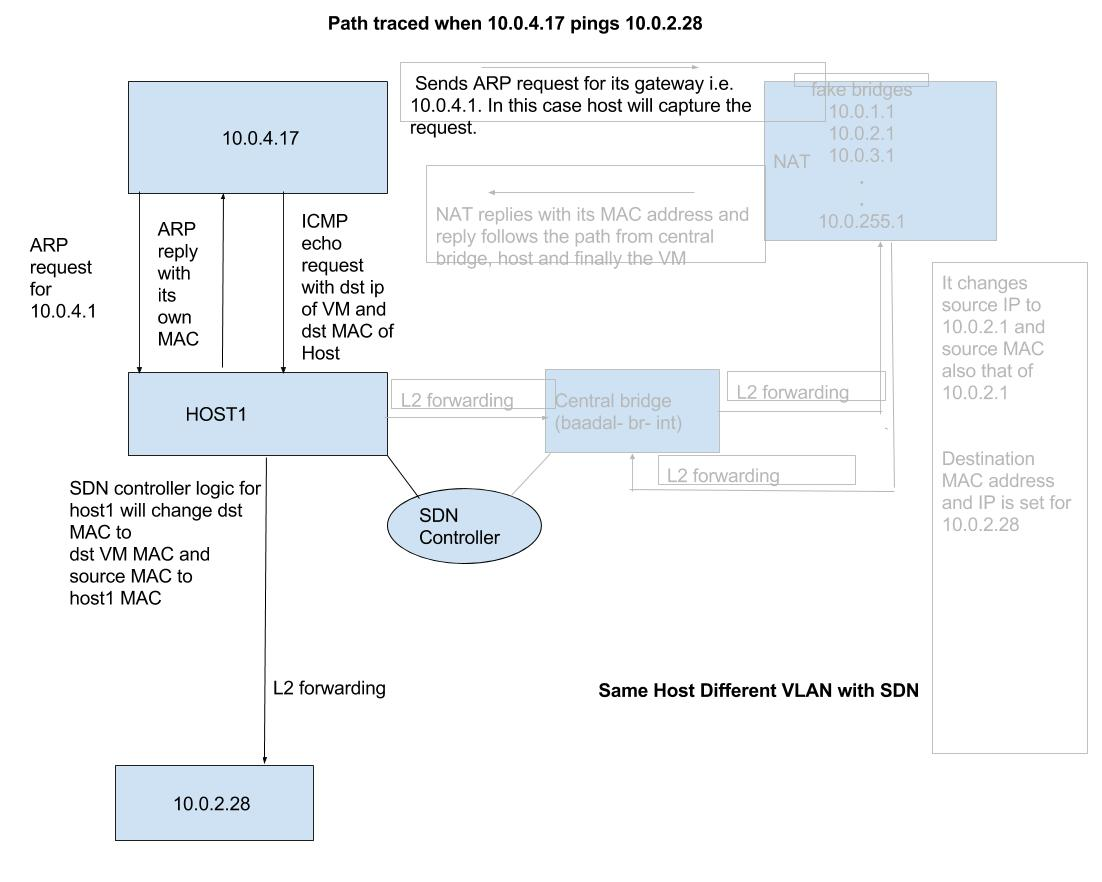
\includegraphics[width=0.9\textwidth]{Samehost_differentvLan_SDN}
\end{figure}

\pagebreak

\begin{itemize}
    \item \textbf{Different host and Different VLAN} In this case host itself will reply to the ARP request, sent by the VM for its gateway. In traditional routing, this reply was generated by the NAT. But now Central bridge will come into the picture to forward the packet to the other host2 unlike previous case. The modification in the Ethernet frame here is done by the host1 only. Host2 will simply forward the packet to the destination VM.
\end{itemize}

\begin{figure}[h]
\caption{Routing in Different Host and Different VLAN using SDN}
\centering
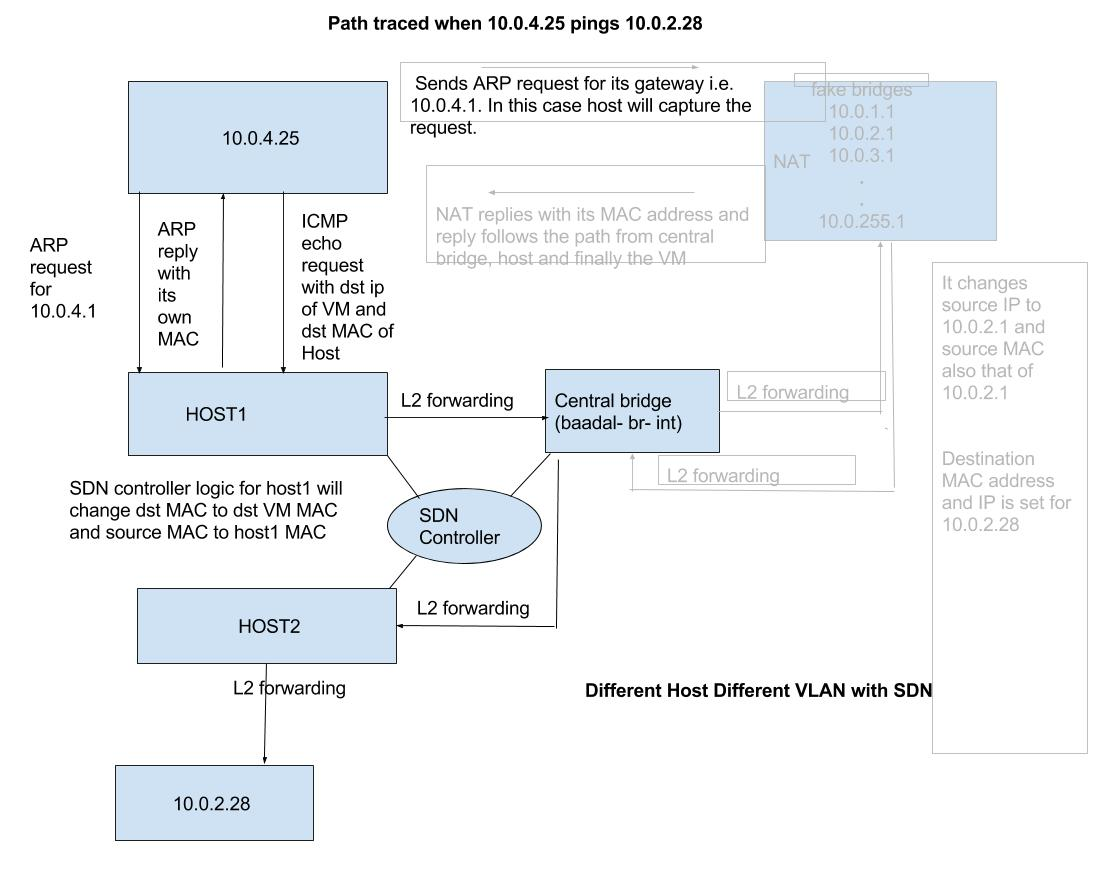
\includegraphics[width=0.9\textwidth]{Differenthost_differentvLan_SDN}
\end{figure}


\pagebreak

\begin{itemize}
    \item \textbf{Different host and Same VLAN} In this, the packet will be forwarded by the host on the basis of the MAC address to the central bridge.The central bridge will further forward it to the other host which subsequently make the packet reach destination VM.
\end{itemize}

\begin{figure}[h]
\caption{Routing in Different Host and Same VLAN using SDN}
\centering
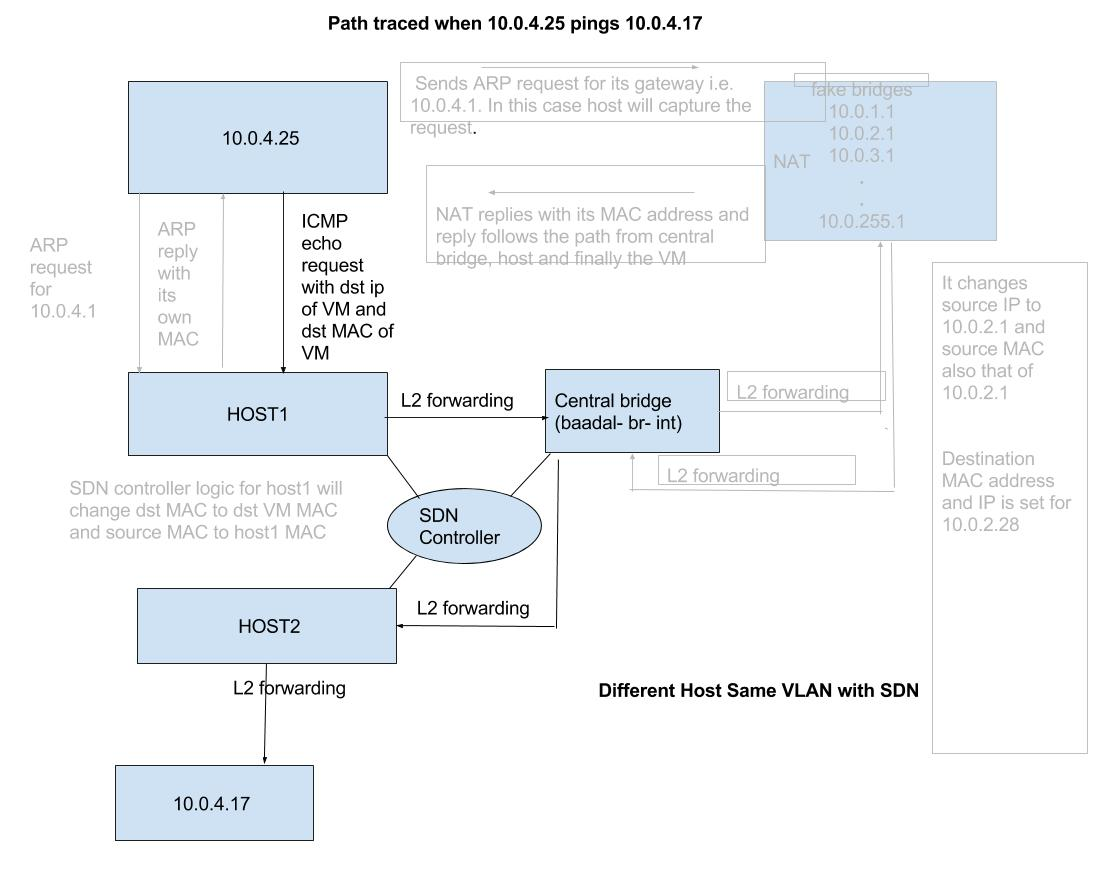
\includegraphics[width=0.9\textwidth]{Differenthost_SamevLan_SDN}
\end{figure}


% \section{Introduction to VMs consolidation application}

% \section{Major issues faced in the project}
\section{Application pseudo code}

\subsection{Hosts}

\begin{algorithm}[H]
\SetAlgoLined


 \If{packet type == IPv6\_TYPE}{
  Drop the packet\;
  Install flow to drop matching packets\;
  }
  \If{packet type== ARP\_TYPE}{
  \If{ARP type == REQUEST}{
    \eIf{destinationProtocolAddress is one of the gateways}{
    send reply with host's mac address\;
    don't send the packet for further processing\;
    }{
    send the packet for further processing\;
    }
  }{
  \If{ARP type == REPLY}{
    store the incoming ip to mac mapping\;
    send the packet for further processing\;
  }
  }
  }
  
  \caption{Handling arp requests at hosts}
  \end{algorithm}
  \newpage
  \begin{algorithm}[H]
  \SetAlgoLined
  
  
  
  \If{input port = local port}{
  \If{mac corresponding to destination ip is not known}
  {
    send ARP request for destination ip\;
    wait for 100ms\;
  }
  \eIf{mac corresponding to destination ip is still not known}
    {drop the packet\;
  }{
   replace the destination mac address of the packet with the mac corresponding to the destination ip read from the table\;
  }
  \eIf{output port is known}
  {
    send the packet out\;
    install flow for all the above actions\;
  }
  {
    drop the packet\;
  }
  }
 \caption{Routing packets coming from local port of hosts}
\end{algorithm}

\newpage
\begin{algorithm}
\SetAlgoLined

\If{input port = trunk port}{
\If{output port corresponding to destination mac is not known}
  {
    send ARP request for destination ip and wait for 100ms\;
  }
  \eIf{output port is still not known}
    {drop the packet\;
  }{
   \eIf{output port is local or trunk}{
     send packet out and install flow\;
   }{
    \eIf{packet is untagged}
    {
        send packet out and install flow\;
    }{
        get policy decision between source and target ip address\;
        \If{decision == ALLOW}{
            pop vlan, send packet out and install flow\;
        }
        \If{decision == DISALLOW}{
            drop packet and install flow\;
        }
        \If{decision == DEFAULT}{
            \eIf{inter vlan routing is enabled}{
                pop vlan, send packet out and install flow\;
            }{
                \If{vlan tag of packet is same destination ip's tag}{
                    pop vlan, send packet out and install flow\;
                }{
                    drop the packet and install flow;
                }
                
            }
        }
    }
   }
  }
}
\caption{Routing packets coming from trunk port of hosts}
\end{algorithm}

\newpage
\begin{algorithm}
%\SetAlgoLined

\If{input port = access port}{
figure out if the packet is intended for the host or for any other machine\;
\eIf{destination ip is NOT of host AND destination mac is of host}{
    \If{mac corresponding to destination ip is not known}
  {
    send ARP request for destination ip\;
    wait for 100ms\;
  }
  \eIf{mac corresponding to destination ip is still not known}
    {drop the packet\;
  }{
    set the destination mac address to the mac corresponding to destination ip from the table\;
    set the source mac to host's mac\;
  }
  \If{output port is not known}{
    send ARP request for destination ip address\;
    wait for 100 ms\;
  }
}{
    \If{output port is not known}{
    send ARP request for destination ip address\;
    wait for 100 ms\;
    }
    \eIf{output port is known}{
        \If{output port is TRUNK}{
            push vlan tag, send packet out and install flow\;
        }
        \If{output port is LOCAL}{
            send packet out and install flow\;
        }
        \If{output port is ACCESS}{
            route according to inter vm policy\;
            check next page for details\;
        }
    }{
        drop packet and install flow\;
    }
}
}
\caption{Routing packets coming from access ports of hosts}
\end{algorithm}

\newpage
\begin{algorithm}
\SetAlgoLined
\If{output port is ACCESS}{
    get policy decision between source and target ip addresses\;
    \If{decision == ALLOW}{
        send packet out and install flow\;
    }
    \If{decision == DISALLOW}{
        drop packet and install flow\;
    }
    \If{decision == DEFAULT}{
        \eIf{inter vlan routing is enabled}{
            send packet out and install flow\;
        }{
            \eIf{vlan tags of source and target ip are same}{
                send packet out and install flow\;
            }{
                drop packet and install flow\;
            }
        }
        
    }
}
\caption{Routing according to inter vm policy when both input and output ports are access ports}
\end{algorithm}